\documentclass{classrep}
\usepackage[utf8x]{inputenc}
\usepackage{color}
\usepackage{environ}
\usepackage{comment}
\usepackage{amsmath}
\usepackage{amssymb}
\usepackage{amsthm}
\usepackage{longtable}
\usepackage{float}
\usepackage{lscape}
\usepackage{icomma}
\usepackage{graphicx}
\usepackage{eurosym}
\usepackage{hyperref}

\newcommand{\card}{\mathrm{card}}
\renewcommand{\labelitemi}{\textbullet}
\renewcommand{\arraystretch}{1.333}
{\theoremstyle{definition}
  \newtheorem{definition}{Definicja}
}

\graphicspath{{graphs}}

\studycycle{Informatyka, studia dzienne, I st.}
\coursesemester{VI}

\coursename{Komputerowe systemy rozpoznawania}
\courseyear{2018/2019}

\courseteacher{dr inż. Marcin Kacprowicz}
\coursegroup{wtorek, 16.15}

\author{
  \studentinfo{Piotr Traczyk}{195733} \and
  \studentinfo{Bartosz Jurczewski}{210209}
}

\title{Zadanie 2: Lingwistyczne podsumowania baz danych}
\svnurl{https://github.com/jurczewski/KSR}

\begin{document}
\maketitle


\section{Cel}
"Zadanie polega na stworzeniu aplikacji desktopowej przy użyciu dowolnego formatu bazy danych. W ogólności, aplikacja ma charakter systemu doradczego, który generuje pewną ilość podsumowań lingwistycznych dla podanej bazy, a następnie przedstawia użytkownikowi wybrane – najlepsze wg zastosowanych miar jakości – wyniki, czyli podsumowania lingwistyczne. Aplikacja umożliwiać ma automatyczne generowanie podsumowań lingwistycznych służących do tworzenia krótkich wiadomości tekstowych na podstawie dużej relacyjnej bazy danych." \cite{tresc}

\section{Wprowadzenie}
Kwestią jaką zajmowaliśmy się w ramach projektu była analiza funkcjonowania lingwistycznych podsumowań baz danych na zbiorach rozmytych. Zbiór rozmyty jest fundamentalnym terminem wykorzystywanym przy naszym projekcie, dlatego też pozwoliliśmy sobie przedstawić jego definicje.

\begin{definition}Niech \(\mathcal{X}\) będzie zbiorem, którego elementy interesują
nas w sposób bezpośredni czyli jest ,,zbiorem zwykłym''.
Wówczas \emph{zbiorem rozmytym opisanym na \(\mathcal{X}\)}
nazywamy każdy zbiór \(A\) postaci:
\[A = \bigcup_{x \in \mathcal{X}} \{(x,\, \mu_A(x))\},\]
gdzie \(\mu_A(x) : \mathcal{X} \to [0,\,1]\) nazywamy \emph{funkcją
przynależności do zbioru rozmytego \(A\)}.
\end{definition}

\textbf{Funkcja przynależności} definiuje w jakim stopniu dany element przynależy do zbioru. W zbiorach rozmytych zakres wartości jakie może ona przyjmować jest rozszerzony do przedziału [0,1]. W naszym projekcie skorzystaliśmy z funkcji przynależności \emph{trójkątnej} oraz \emph{trapezoidalnej}. Ich definicje są następujące:

\begin{definition}[Zbiór rozmyty o trójkątnej funkcji przynależności]
Zbiór rozmyty \(A\) opisany na przestrzeni \(\mathbb{R}\) jest
\emph{liczbą rozmytą trójkątną o parametrach \(a, b, c\)} wtedy i tylko
wtedy, gdy \(a \leq b \leq c\) oraz:

\[\mu_A(x) = \begin{cases}
0                 & \mbox{gdy } x \in (-\infty,\, a], \\
(x - a) / (b - a) & \mbox{gdy } x \in (a,\, b), \\
1                 & \mbox{gdy } x = b, \\
(c - x) / (c - b) & \mbox{gdy } x \in (b,\, c), \\
0                 & \mbox{gdy } x \in [c,\, +\infty).
\end{cases}\]
\end{definition}

\vspace\baselineskip

\begin{definition}[Zbiór rozmyty o trapezoidalnej funkcji przynależności]
Zbiór rozmyty \(A\) opisany na przestrzeni \(\mathbb{R}\) jest
\emph{liczbą rozmytą trapezoidalną o parametrach \(a, b, c, d\)} wtedy i tylko
wtedy, gdy \(a \leq b \leq c \leq d\) oraz:

\[\mu_A(x) = \begin{cases}
0                 & \mbox{gdy } x \in (-\infty,\, a], \\
(x - a) / (b - a) & \mbox{gdy } x \in (a,\, b), \\
1                 & \mbox{gdy } x \in [b,\, c], \\
(d - x) / (d - c) & \mbox{gdy } x \in (c,\, d), \\
0                 & \mbox{gdy } x \in [d,\, +\infty).
\end{cases}\]
\end{definition}

\vspace\baselineskip

\begin{figure}[H]
	\centering
	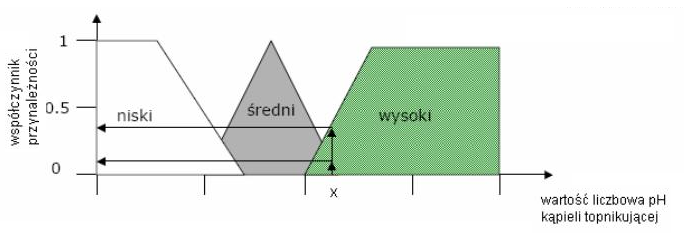
\includegraphics[width=1\textwidth]{{/przyklad_funkcji.png}}
	\caption{Przykład funkcji przynależności - trójkątnej oraz trapezoidalnej \cite{funkcje}}
\end{figure}

\section{Opis implementacji}
Program został stworzony przy użyciu .NET Framework w języku C\#. Graficzny interfejs powstał przy wykorzystaniu Windows Presentation Foundation. Cały projekt został napisany zgodnie ze wzorcem architektonicznym Model–view–viewmodel (MVVM), w związku z tym powstały trzy warstwy Logic, ViewModel i GUI.

\subsection{Logic}
Warstwa odpowiedzialna za logikę aplikacji. Klasa reprezentująca krotkę w bazie (\emph{Player.cs}), zaimplementowane zostały: funkcje przynależności trójkątna (\emph{TriangularFunction.cs}) oraz trapezoidalna (\emph{TrapezoidFunction}), zmienna lingwistyczna (\emph{LinguisticVariable.cs}), kwantyfikator (\emph{StaticQuantifiers.cs}), zmienna, która ”na sztywno” określa nasz kwantyfikator (np. słaby, przeciętny, dobry) w zależności od podanych danych (\emph{StaticVariables.cs}), sumaryzator ”i” (\emph{And.cs}), a także sumaryzator ”lub” (\emph{Or.cs}). W tej warstwie znajduje się także klasa (\emph{Measures.cs}), gdzie zawarliśmy wszystkie 11 miar jakości podsumowań.
\subsection{ViewModel}
Klasa MainViewModel przyjmuje dane wejściowe od użytkownika i reaguje na jego poczynania wywołując wybrane akcje z logiki programu oraz odpowiada za odświeżanie widoków w interfejsie graficznym.
\subsection{GUI}
Przejrzysty interfejs użytkownika który ma kontrole nad kwalifikatorem, sumaryzatorem (również złożonym OR/AND), generowaniem podsumowań oraz zapisem do pliku.

\section{Miary jakości}
Do określenia jakości podsumowania lingwistycznego zaimplementowaliśmy następujące miary jakości, których wzory zostały zaczerpnięte z \cite{adam}.
\begin{itemize}
    \item $T_1$ (\emph{Degree of truth}) - Suma przynależności wszystkich rozważanych krotek do podsumowania lingwistycznego.
    \item $T_2$ (\emph{Degree of imprecision}) - Określa stopień precyzyjności sumaryzatora (miarę jakości podsumowania).
    \item $T_3$ (\emph{Degree of covering}) - Reprezentuje stopień w jakim nośnik sumaryzatora pokrywa się z nośnikiem kwalifikatora.
    \item $T_4$ (\emph{Degree of appropriateness}) - Definiuje jak dużo krotek przynależy do sumaryzatora, czyli czy określone podsumowanie jest odpowiednie dla zestawu danych.
    \item $T_5$ (\emph{Length of summary}) - Określa jakość podsumowania na podstawie złożoności sumaryzatora, dając prostą zależność - im więcej składowych sumaryzatora złożonego, tym mniejsza wartość tej miary.
    \item $T_6$ (\emph{Degree of quantifier imprecision}) - Pokazuje w jakim stopniu precyzyjny jest kwantyfikator. Im mniejszy nośnik zbioru rozmytego tym wyższa jest jego precyzja.
    \item $T_7$ (\emph{Degree of quantifier cardinality}) - Opisuje stopień precyzji kwantyfikatora, im mniejsza kardynalność kwantyfikatora tym jest on bardziej precyzyjny.
    \item $T_8$ (\emph{Degree of summarizer cardinality}) - Opisuje stopień precyzji sumaryzatora, im mniejsza kardynalność kwantyfikatora tym jest on bardziej precyzyjny.
    \item $T_9$ (\emph{Degree of qualifier imprecision}) - Określa w jakim stopniu precyzyjny jest kwalifikator. Im szerszy nośnik zbioru rozmytego tym niższa jest jego precyzja, gdyż bierze pod uwagę większy zakres wartości.
    \item $T_{10}$ (\emph{Degree of qualifier cardinality}) - Opisuje stopień precyzji kwalifikatora, im większa jest kardynalność kwalifikator tym jest on mniej precyzyjny.
    \item $T_{11}$ (\emph{Length of qualifier}) - Wyznacza jakość podsumowania na podstawie złożoności kwalifikatora. Im bardziej złożony kwalifikator tym jakość podsumowania gorsza.
\end{itemize}
\section{Materiały i metody}
\subsection{Baza danych}
Do realizacji zadania wybraliśmy bazę danych \emph{Fifa 19} \cite{data}. Wybrana baza
składa się z \(18128\) krotek znajdujących się w tabeli z \(10\) kolumnami różnych typów. Przechowuje ona statystyki piłkarzy z gry Fifa 2019.\\ Do tworzenia podsumowań
korzystamy z kolumn:
\begin{itemize}
    \item Age - wiek [Lata]
    \item Overall - ocena całkowita zawodnika
    \item Value - wartość zawodnika [\euro]
    \item Wage - zarobki [\euro]
    \item Height - wzrost [Stopy i Cale]
    \item Weight - waga [Funty]
    \item FKAccuracy - (free kicks accuracy) - efektywność rzutów wolnych (procent bramek z rzutów wolnych)
    \item SprintSpeed - szybkość w sprincie
    \item Stamina - wytrzymałość
    \item Strength - siła
\end{itemize}

\begin{figure}[H]
    \centering
    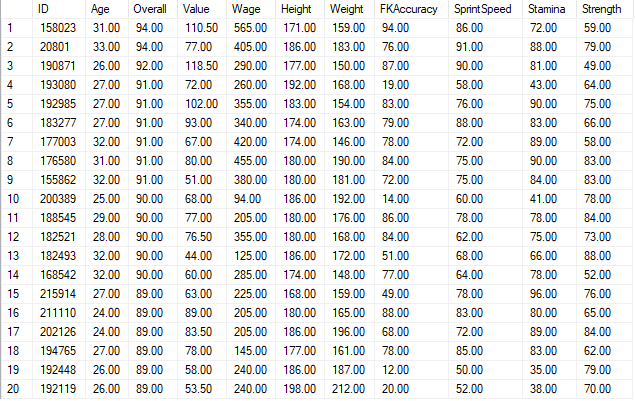
\includegraphics[width=13cm]{/select_baza.png}
    \caption{Fragment widoku tabeli}
\end{figure}
\subsection{Sumaryzatory i kwalifikatory}
Poniżej zaprezentowaliśmy poszczególne sumaryzatory oraz kwalifikatory wykorzystane w naszym programie. 

\begin{table}[H]
	\centering
	\begin{tabular}{c c c c c} 
		\hline
		\textbf{Etykieta} & \textbf{a} & \textbf{b} & \textbf{c} &  \textbf{d} \\ [0.5ex] 
		\hline
		\hline 
		Young & 15 & 16 & 17 & 20 \\ 
		Adult & 19 &  23 &  27 &  31 \\
		Old &  30 &  35 &  45 &  51 \\
		\hline
	\end{tabular}
	\caption{Przyporządkowane parametry funkcji trapezoidalnej dla wieku.}
\end{table}

\begin{table}[H]
	\centering
	\begin{tabular}{c c c c c} 
		\hline
		\textbf{Etykieta} & \textbf{a} & \textbf{b} & \textbf{c} &  \textbf{d} \\ [0.5ex] 
		\hline
		\hline 
		Low Overall & 46 &  50 &  55 &  60\\
		Medium Overall & 59 &  64 &  70 &  75\\
		Good Overall &   74 &  80 &  85 &  94 \\
		\hline
	\end{tabular}
	\caption{Przyporządkowane parametry funkcji trapezoidalnej dla wyniku ogólnego.}
\end{table}

\begin{table}[H]
	\centering
	\begin{tabular}{c c c c c} 
		\hline
		\textbf{Etykieta} & \textbf{a} & \textbf{b} & \textbf{c}  \\ [0.5ex] 
		\hline
		\hline 
		Low Value & 0 &  30 &  60 &  100 \\ 
		Medium Value & 99 &  200 &  400 &  600 \\
		High Value &  599 &  750 &  850 &  975 \\
		\hline
	\end{tabular}
	\caption{Przyporządkowane parametry funkcji trapezoidalnej dla wartości piłkarza.}
\end{table}

\begin{table}[H]
	\centering
	\begin{tabular}{c c c c c} 
		\hline
		\textbf{Etykieta} & \textbf{a} & \textbf{b} & \textbf{c}  \\ [0.5ex] 
		\hline
		\hline 
		Low Wage & 0 &  2 &  4 &  6 \\ 
		Medium Wage & 5 &  7 &  9 &  12 \\
		High Wage &  11 &  50 &  90 &  110 \\
		Very High Wage &  109 &  250 &  400 &  565 \\
		\hline
	\end{tabular}
	\caption{Przyporządkowane parametry funkcji trapezoidalnej dla zarobków.}
\end{table}

\begin{table}[H]
	\centering
	\begin{tabular}{c c c c c} 
		\hline
		\textbf{Etykieta} & \textbf{a} & \textbf{b} & \textbf{c}  \\ [0.5ex] 
		\hline
		\hline 
		Short & 153 &  160 & 167 & 172 \\ 
		Medium HeightTall & 171 & 176 & 181 & 185 \\
		Tall & 184 & 190 & 200 & 207 \\
		\hline
	\end{tabular}
	\caption{Przyporządkowane parametry funkcji trapezoidalnej dla wzrostu.}
\end{table}

\begin{table}[H]
	\centering
	\begin{tabular}{c c c c c} 
		\hline
		\textbf{Etykieta} & \textbf{a} & \textbf{b} & \textbf{c}  \\ [0.5ex] 
		\hline
		\hline 
		Light & 110 & 110 & 150 & 155 \\ 
		Regular & 150 & 160 & 190 & 200 \\
		Heavy & 195 & 210 & 240 & 255 \\
		\hline
	\end{tabular}
	\caption{Przyporządkowane parametry funkcji trapezoidalnej dla wagi.}
\end{table}


\begin{table}[H]
	\centering
	\begin{tabular}{c c c c c} 
		\hline
		\textbf{Etykieta} & \textbf{a} & \textbf{b} & \textbf{c}  \\ [0.5ex] 
		\hline
		\hline 
		Bad Free Kick & 3 & 15 & 30 & 40 \\ 
		Decent Free Kick & 39 & 46 & 58 & 70 \\
		Good Free Kick & 69 & 75 & 87 & 94 \\
		\hline
	\end{tabular}
	\caption{Przyporządkowane parametry funkcji trapezoidalnej dla FKAccuracy.}
\end{table}

\begin{table}[H]
	\centering
	\begin{tabular}{c c c c c} 
		\hline
		\textbf{Etykieta} & \textbf{a} & \textbf{b} & \textbf{c}  \\ [0.5ex] 
		\hline
		\hline 
		Bad Sprint & 12 & 20 & 30 & 40 \\ 
		Decent Sprint & 39 & 47 & 58 & 68 \\
		Good Sprint & 67 & 75 & 85 & 96 \\
		\hline
	\end{tabular}
	\caption{Przyporządkowane parametry funkcji trapezoidalnej dla szybkości sprintu.}
\end{table}

\begin{table}[H]
	\centering
	\begin{tabular}{c c c c c} 
		\hline
		\textbf{Etykieta} & \textbf{a} & \textbf{b} & \textbf{c}  \\ [0.5ex] 
		\hline
		\hline 
		Bad Stamina & 12 & 19 & 31 & 40 \\ 
		Decent Stamina & 39 & 45 & 57 & 68 \\
		Good Stamina & 67 & 75 & 87 & 96 \\
		\hline
	\end{tabular}
	\caption{Przyporządkowane parametry funkcji trapezoidalnej dla wytrzymałości.}
\end{table}

\begin{table}[H]
	\centering
	\begin{tabular}{c c c c c} 
		\hline
		\textbf{Etykieta} & \textbf{a} & \textbf{b} & \textbf{c}  \\ [0.5ex] 
		\hline
		\hline 
		Bad Strength & 17 & 25 & 36 & 45 \\ 
		Decent Strength & 54 & 65 & 74 & 80 \\
		Good Strength & 79 & 85 & 90 & 97 \\
		\hline
	\end{tabular}
	\caption{Przyporządkowane parametry funkcji trapezoidalnej dla siły.}
\end{table}

\subsection{Kwantyfikatory}
\begin{table}[H]
	\centering
	\begin{tabular}{c c c c c c} 
		\hline
		\textbf{Etykieta} & \textbf{Funkcja przynależności} & \textbf{a} & \textbf{b} & \textbf{c} &  \textbf{d} \\ 
		\hline
		\hline 
		No & Trójkątna & 0 & 0 & 0.16 & - \\
		Around 20\% & Trójkątna & 0.14 & 0.2 & 0.26& - \\
		Around one third & Trójkątna & 0.25 &  0.33 &  0.41 & - \\
	    Less than a third & Trapezoidalna & 0 &  0 &  0.3 &  0.36\\
		Around 40\% & Trójkątna &  0.34 &  0.4 &  0.46 & - \\
		Around half & Trójkątna & 0.4 &  0.5 &  0.6 & - \\
		Around three quaters & Trójkątna &  0.5 &  0.6 &  0.7 & - \\
		Majority & Trójkątna & 0.75 &  0.8 &  0.9 & -  \\
		All & Trapezoidalna & 0.85 &  0.9 &  1 &  1 \\
		\hline
	\end{tabular}
	\caption{Przyporządkowane parametry dla kwantyfikatora względnego.}
\end{table}

\begin{table}[H]
	\centering
	\begin{tabular}{c c c c c c} 
		\hline
		\textbf{Etykieta} & \textbf{Funkcja przynależności} & \textbf{a} & \textbf{b} & \textbf{c} &  \textbf{d} \\ 
		\hline
		\hline 
		Less than 1000 & Trapezoidalna & 0 & 0 & 9990 & 1000 \\ 
		Around 1500 & Trójkątna & 1400 & 1500 & 1600 & - \\
		Around 3000 & Trójkątna & 2900 & 3000 & 3100 & - \\
		More than 5000 & Trapezoidalna & 5000 & 5010 & 5500 & - \\
		\hline
	\end{tabular}
	\caption{Przyporządkowane parametry dla kwantyfikatora absolutnego.}
\end{table}

\section{Badania}
Nasze badania postanowiliśmy podzielić na trzy części:
\begin{enumerate}
    \item Sprawdzenie jakie wartości przybiorą miary podsumowań dla różnych kwantyfikatorów. 
    \item Porównanie podsumowań bez i z kwalifikatorem.
    \item Porównanie podsumowań z jednym sumaryzatorem oraz połączanie ze spójnikami OR i LUB.
\end{enumerate}

\subsection{Pierwszy eksperyment}
W tym badaniu wygenerowaliśmy 3 komunikaty, dotyczące odpowiednio zależności pomiędzy:
\begin{itemize}
    \item 'BodyweightKg' a 'Sprint Speed'
    \item 'Height' a 'Wage'
\end{itemize}
Miary $T_2-T_5$ oraz $T_8-T{10}$ były stałe dla różnych kwalifikatorów dlatego zostały przez nas pominięte w tabeli oraz na wykresie, ponieważ kwantyfikator nie miał wpływu na ich wartość. Zostały jednak przedstawione pod tabelą porównującą wartości miar $T_1$, $T_6$ i $T_7$. 
\subsubsection{Eksperyment 1.1}

\begin{figure}[H]
	\centering
	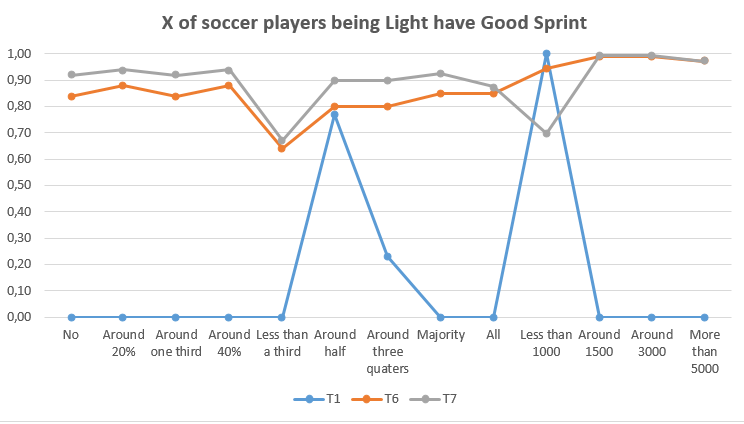
\includegraphics[width=1\textwidth]{{/Badanie11.png}}
	\caption{Wykres przedstawiający wyniki Eksperymentu 1.1}
\end{figure}

\begin{table}[H]
	\centering
	\begin{tabular}{c c c c} 
		\hline
		\textbf{Kwantyfikator} & \textbf{$T_1$} & \textbf{$T_6$} & \textbf{$T_7$}\\ [0.5ex] 
		\hline
		\hline 
        No & 0,00 & 0,84 & 0,92\\
        Around 20\% & 0,00 & 0,88 & 0,94\\
        Around one third & 0,00 & 0,84 & 0,92\\
        Around 40\% & 0,00 & 0,88 & 0,94\\
        Less than a third & 0,00 & 0,64 & 0,67\\
        Around half & 0,77 & 0,80 & 0,90\\
        Around three quaters & 0,23 & 0,80 & 0,90\\
        Majority & 0,00 & 0,85 & 0,93\\
        All & 0,00 & 0,85 & 0,88\\
        Less than 1000 & 1,00 & 0,94 & 0,70\\
        Around 1500 & 0,00 & 0,99 & 0,99\\
        Around 3000 & 0,00 & 0,99 & 0,99\\
        More than 5000 & 0,00 & 0,97 & 0,97\\
		\hline
	\end{tabular}
	\caption{Tabela przedstawiający wyniki Eksperymentu 1.1}
\end{table}

Uzyskane miary, które były jednakowe dla każdego kwantyfikatora: $T_2 = 0.508$, $T_3 = 0.669$, $T_4 = 0.669$, $T_5 = 1$, $T_8 = 0.999$, $T_9 = 0.728$, $T_{10} = 0.998$, $T_{11} = 1$.

\subsubsection{Eksperyment 1.2}

\begin{figure}[H]
	\centering
	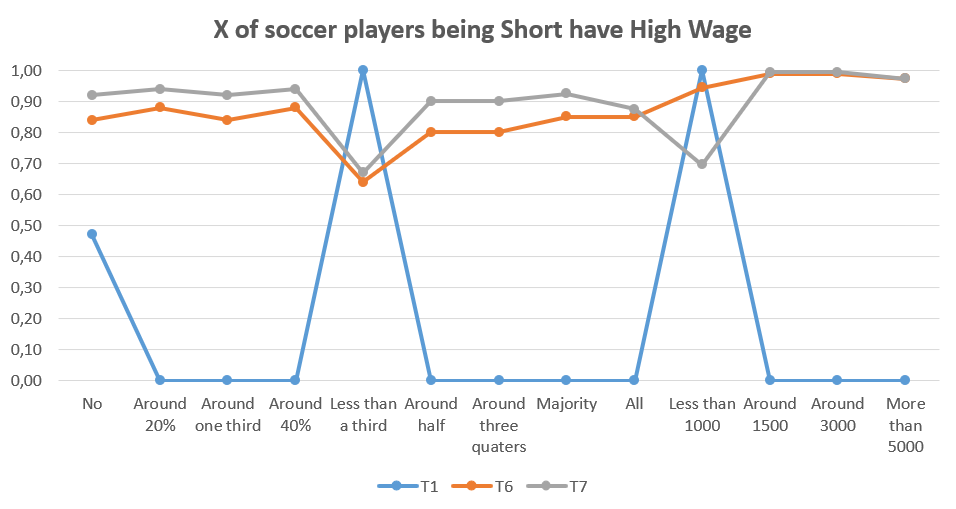
\includegraphics[width=1\textwidth]{{/Badanie12.png}}
	\caption{Wykres przedstawiający wyniki Eksperymentu 1.2}
\end{figure}

\begin{table}[H]
	\centering
	\begin{tabular}{c c c c} 
		\hline
		\textbf{Kwantyfikator} & \textbf{$T_1$} & \textbf{$T_6$} & \textbf{$T_7$}\\ [0.5ex] 
		\hline
		\hline 
        No & 0,47 & 0,84 & 0,92\\
        Around 20\% & 0,00 & 0,88 & 0,94\\
        Around one third & 0,00 & 0,84 & 0,92\\
        Around 40\% & 0,00 & 0,88 & 0,94\\
        Less than a third & 1,00 & 0,64 & 0,67\\
        Around half & 0,00 & 0,80 & 0,90\\
        Around three quaters & 0,00 & 0,80 & 0,90\\
        Majority & 0,00 & 0,85 & 0,93\\
        All & 0,00 & 0,85 & 0,88\\
        Less than 1000 & 1,00 & 0,94 & 0,70\\
        Around 1500 & 0,00 & 0,99 & 0,99\\
        Around 3000 & 0,00 & 0,99 & 0,99\\
        More than 5000 & 0,00 & 0,97 & 0,97\\
        \hline
	\end{tabular}
	\caption{Tabela przedstawiający wyniki Eksperymentu 1.1}
\end{table}

Uzyskane miary, które były jednakowe dla każdego kwantyfikatora: $T_2 = 0.804$, $T_3 = 0.189$, $T_4 = 0.189$, $T_5 = 1$, $T_8 = 0.996$, $T_9 = 0.922$, $T_{10} = 0.999$, $T_{11} = 1$.

\subsection{Drugi eksperyment}
W tym badaniu wygenerowaliśmy podsumowanie dotyczące FK Accuracy. Sprawdziliśmy jak obecność kwalifikatora (Age: Adult) wpłynęła na wartości miar.
Miary $T_9-T_{11}$ zależały od kwalifikatora - nie dało się ich obliczyć bez niego, dlatego nie były porównywane w tym badaniu.
\subsubsection{Eksperyment 2.1}
\begin{figure}[H]
	\centering
	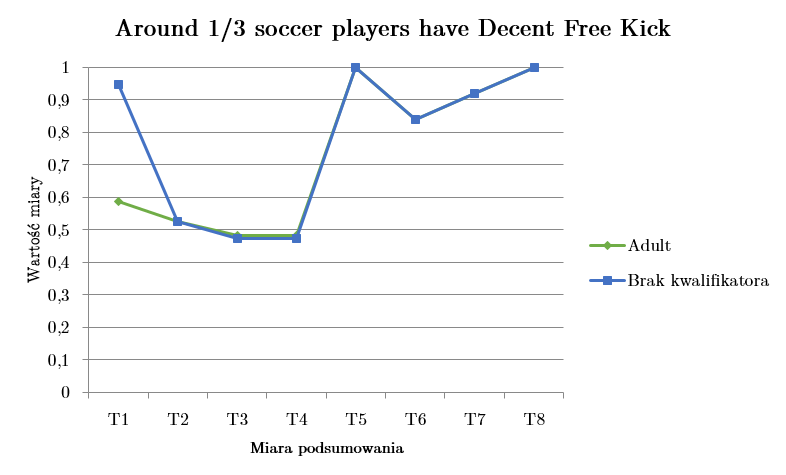
\includegraphics[width=1\textwidth]{/Badanie211.png}
	\caption{Wykres przedstawiający wyniki Eksperymentu 2.1 - kwantyfikator względny}
\end{figure}

\begin{table}[H]
	\centering
	\begin{tabular}{c c c} 
		\hline
		\textbf{Miara} & \textbf{Adult} & \textbf{Brak kwalifikatora}\\ [0.5ex] 
		\hline
		\hline 
        $T_1$ & 0,587 & 0,948\\
        $T_2$ & 0,527 & 0,527\\
        $T_3$ & 0,484 & 0,473\\
        $T_4$ & 0,484 & 0,473\\
        $T_5$ & 1,000 & 1,000\\
        $T_6$ & 0,840 & 0,840\\
        $T_7$ & 0,920 & 0,920\\
        $T_8$ & 0,999 & 0,999\\
		\hline
	\end{tabular}
	\caption{Tabela przedstawiająca wyniki Eksperymentu 2.1 - kwantyfikator względny (około 1/3 piłkarzy)}
\end{table}

\begin{figure}[H]
	\centering
	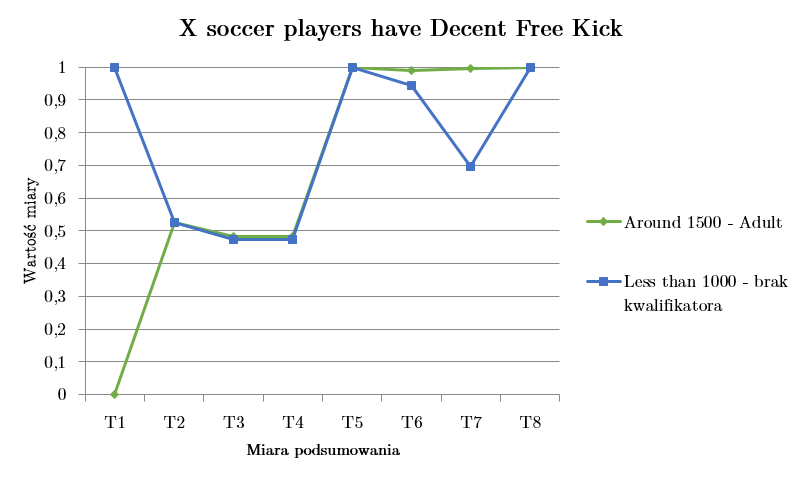
\includegraphics[width=1\textwidth]{/Badanie212.png}
	\caption{Wykres przedstawiający wyniki Eksperymentu 2.1 - kwantyfikator bezwzględny}
\end{figure}

\begin{table}[H]
	\centering
	\begin{tabular}{c c c } 
		\hline
		& \textbf{Adult} & \textbf{Brak kwalifikatora}\\ [0.5ex]
		\textbf{Miara} & \textbf{Around 1500} & \textbf{Less than 1000}\\ [0.5ex]
		\hline
		\hline 
        $T_1$ & 0,000 & 1,000\\
        $T_2$ & 0,527 & 0,527\\
        $T_3$ & 0,484 & 0,473\\
        $T_4$ & 0,484 & 0,473\\
        $T_5$ & 1,000 & 1,000\\
        $T_6$ & 0,989 & 0,945\\
        $T_7$ & 0,994 & 0,697\\
        $T_8$ & 0,999 & 0,999\\
		\hline
	\end{tabular}
	\caption{Tabela przedstawiająca wyniki Eksperymentu 2.1 - kwantyfikator bezwzględny}
\end{table}

\subsection{Trzeci eksperyment}
W tym badaniu wygenerowaliśmy podsumowania dotyczące dorosłych piłkarzy, którzy mają:
\begin{itemize}
    \item Bad Strength
    \item Bad Stamina
    \item Bad Strength AND Bad Stamina
    \item Bad Strength OR Bad Stamina
\end{itemize}

\begin{figure}[H]
	\centering
	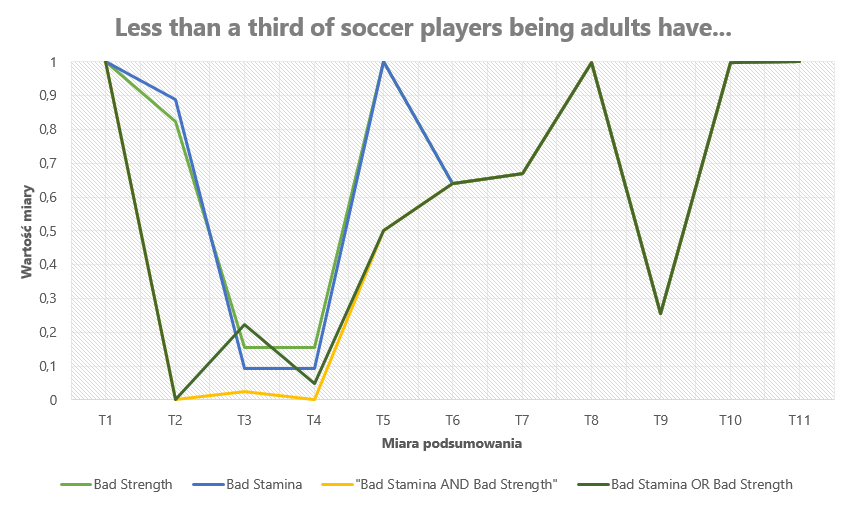
\includegraphics[width=1\textwidth]{/Badanie31.png}
	\caption{Wykres przedstawiający wyniki Eksperymentu 3 - kwantyfikator względny}
\end{figure}


\begin{table}[H]
	\centering
	\begin{tabular}{c c c c c } 
		\hline
		\textbf{Miara} & \textbf{Bad Strength} & \textbf{Bad Stamina} & \textbf{ORAZ} & \textbf{LUB}\\ [0.5ex] 
		\hline
		\hline 
            $T_1$ & 1,00 & 1,00 & 1,00 & 1,00\\
            $T_2$ & 0,82 & 0,89 & 0,00 & 0,00\\
            $T_3$ & 0,16 & 0,09 & 0,03 & 0,22\\
            $T_4$ & 0,16 & 0,09 & 0,00 & 0,05\\
            $T_5$ & 1,00 & 1,00 & 0,50 & 0,50\\
            $T_6$ & 0,67 & 0,67 & 0,67 & 0,67\\
            $T_7$ & 0,67 & 0,67 & 0,67 & 0,67\\
            $T_8$ & 1,00 & 1,00 & 1,00 & 1,00\\
            $T_9$ & 0,26 & 0,26 & 0,26 & 0,26\\
            $T_{10}$ & 1,00 & 1,00 & 1,00 & 1,00\\
            $T_{11}$ & 1,00 & 1,00 & 1,00 & 1,00\\
		\hline
	\end{tabular}
	\caption{Tabela przedstawiająca wyniki Eksperymentu 3 - kwantyfikator względny (mniej niż 1/3 dorosłych piłkarzy)}
\end{table}

\begin{figure}[H]
	\centering
	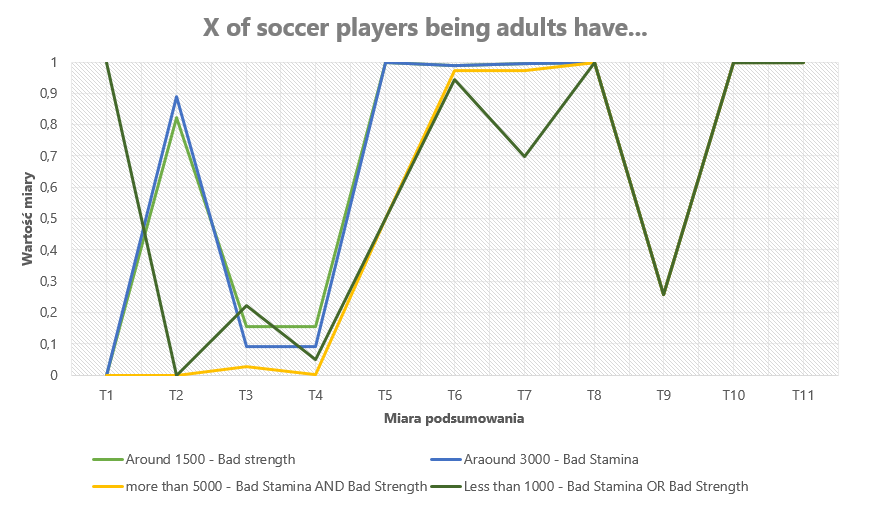
\includegraphics[width=1\textwidth]{/Badanie32.png}
	\caption{Wykres przedstawiający wyniki Eksperymentu 3 - kwantyfikator względny}
\end{figure}


\begin{table}[H]
	\centering
	\begin{tabular}{c c c c c } 
		\hline
		& \textbf{Bad Strength} & \textbf{Bad Stamina} & \textbf{ORAZ} & \textbf{LUB}\\ [0.5ex] 
		\textbf{Miara} & \textbf{Around 1500} & \textbf{Around 3000} & \textbf{More than 5000} & \textbf{More than 1000}\\ [0.5ex] 
		\hline
		\hline 
            $T_1$ & 0,00 & 0,00 & 0,00 & 1,00\\
            $T_2$ & 0,82 & 0,89 & 0,00 & 0,00\\
            $T_3$ & 0,16 & 0,09 & 0,03 & 0,22\\
            $T_4$ & 0,16 & 0,09 & 0,00 & 0,05\\
            $T_5$ & 1,00 & 1,00 & 0,50 & 0,50\\
            $T_6$ & 0,99 & 0,99 & 0,97 & 0,70\\
            $T_7$ & 0,99 & 0,99 & 0,97 & 0,70\\
            $T_8$ & 1,00 & 1,00 & 1,00 & 1,00\\
            $T_9$ & 0,26 & 0,26 & 0,26 & 0,26\\
            $T_{10}$ & 1,00 & 1,00 & 1,00 & 1,00\\
            $T_{11}$ & 1,00 & 1,00 & 1,00 & 1,00\\
		\hline
	\end{tabular}
	\caption{Tabela przedstawiająca wyniki Eksperymentu 3 - kwantyfikator bezwzględny}
\end{table}

\section{Dyskusja}

\subsection{Wpływ kwantyfikatora na miary}
Miara $T_1$ (pokazująca prawdziwość danego podsumowania) zmieniała się w zależności do kwantyfikatora. Wykresy z eksperymentu 1.1 jak i 1.2 pokazują dla których kwantyfikatorów to podsumowanie jest trafne. W pierwszym (being Light have Good Sprint) widzimy że jest to względne "Around half" i bezwględne "Less than 1000". W drugim (being Short have High Wage) jest to odpowiednio "Less than a third" i "Less than 1000". Dla kwantyfikatorów "sąsiadów" miara ta zmierzała ku zerze. Dla reszty po prostu wynosiła zero.\\
\newline
Miary $T_6$ i $T_7$ opisują precyzyjność kwantyfikatora. Dla opisanych wyżej kwantyfikatorów przyjmowały one bardzo wysokie wartości (około 0.9) chociaż potrafiły zejść do 0.7.\\
\newline
Miary $T_2-T_5$ oraz $T_8-T_{11}$ nie zmieniały swoich wartości w zależności od użytego kwantyfikatora, co wprost wynika z braku wykorzystania kwantyfikatora w tych wzorach. 
\subsection{Wpływ kwalifikatora na miary}
Największą różnicą miedzy eksperymentami była zmiana miary $T_1$ przy braku lub obecności kwalifikatora. W naszej ocenie porównywanie jednak jej wyników jest bezcelowe - ponieważ pracuję się wtedy na zupełnie innych zbiorach. Przykładowo różnica miedzy $T_1$ z i bez kwalifikatora równa 1.0 skutkowała wahaniami dla miar $T_6$ i $T_7$. \\
\newline
Miara $T_4$ mówi o tym, jak wiele krotek przynależy do sumaryzatora. Ze względu na $T_3$ we wzorze, jej wartość się zmienia, jednakże jej wpływ omówimy w dalszej części opracowania badań.\\
\newline
Miary $T_2, T_5$ oraz $T_8$ nie zmieniały swoich wartości w obrębie jednego eksperymentu, gdyż zależą od sumaryzatora, a nie kwalifikatora. 
\subsection{Wpływ sumaryzatora na miary}
Miara $T_2$ określa stopień precyzyjności sumaryzatora. Biorąć pod uwagę ten jak i poprzednie eksperymenty można z stwierdzić że miara jest tym większa im bardziej precyzyjny jest użyty sumaryzator. W naszym przypadku precyzyjny okazał sie "Bad Stamina", "Bad Strength" ale już nie "Decetn Free Kick".\\
\newline
Miara $T_3$ reprezentuje stopień w jakim nośnik sumaryzatora pokrywa się z nośnikiem kwalifikatora. U nas jest najwyższa dla "Bad Stamina OR Bad Strength" natomiast bliska zeru dla "AND".\\
\newline
Miara $T_4$ mówi o tym ile krotek należy do sumaryzatora. Określa ona jak bardzo podsumowane wartości pasują do zbioru danych. Dla wszystkich 8 pomiarów jej wartości plasowały się w poniżej 0.2, osiągając 0.0 dla "Bad Stamina AND Bad Strength".\\
\newline
Miara $T_5$ zależy od ilości sumaryzatorów. Dla jednego sumaryzatora osiąga wartość 1, zaś dla dwóch - wartość 0.5. Wraz ze zwiększeniem liczby sumaryzatorów jej wartość by malała.\\
\newline
Miara $T_8$ opisująca precyzyjność sumaryzatora dla wszystkich przeprowadzonych przez nas eksperymentów uzyskiwała wartości bardzo bliskie bądź równe 1. 

\section{Wnioski}
\begin{itemize}
    \item Lingwistyczne podsumowania baz danych znacznie przyspieszają analizę dużych zbiorów danych z wieloma atrybutami, dzięki generowaniu prostych i zrozumiałych informacji jej dotyczących.
    \item Liczba krotek w bazie danych bezpośrednio przekłada się precyzyjność podsumowania.
    \item Duża cześć wygenerowanych podsumowań która pokazuje proste zależności, była łatwa do odgadnięcia przed rozpoczęciem badań. Jednakże omawiane metody (i nasza implementacja) dostarcza formalnej statystycznej miary, dzięki czemu wyrażone w języku naturalnym mają poparcie naukowe.
    \item Należy tak dobrać zbiory rozmyte etykiet aby się nakładały. Dzięki czemu pozbywamy się pustych obszarów dziedziny.
    \item Dobrą praktyką są wąskie wartości przy funkcjach przynależności, osiągamy wtedy bardziej miarodajne wyniki.
    \item Miara $T_1$ powinna być jako pierwsza brana pod uwagę. Dopiero przy osiągnięciu wartości dodatnich, powinniśmy przejść do analizy innych miar.
\end{itemize}

\begin{thebibliography}{}
  \bibitem{tresc}
    A. Niewiadomski,
    \emph{Komputerowe Systemy Rozpoznawania: Materiały, przykłady i ćwiczenia do przedmiotu}.
    21 września 2009.
    \url{http://ics.p.lodz.pl/~aniewiadomski/ksr/ksr-projekt2.pdf}
    \bibitem{data}
    Baza danych - "FIFA 19 complete player dataset":\\
    \url{https://www.kaggle.com/karangadiya/fifa19}    
  \bibitem{zadeh}
    L. A. Zadeh,
    \emph{A fuzzy-set-theoretical interpretation of linguistic hedges}.
    Journal of Cybernetics 1972; 2: 4–34.
  \bibitem{adam}
    A. Niewiadomski,
    \emph{Methods for the Linguistic Summarization of Data: Applications of Fuzzy Sets and Their Extensions}.
    Akademicka Oficyna Wydawnicza EXIT,
    Warszawa 2008.
\bibitem{funkcje}
    \url{http://zsi.tech.us.edu.pl/~nowak/si/w2_2013.pdf}
\end{thebibliography}
\end{document}
